\documentclass{article}
\usepackage{graphicx}
\usepackage{subfigure}
\usepackage{multirow}
\usepackage{wrapfig}
\usepackage{amssymb}
\usepackage{amsfonts, amsmath}
\usepackage{amsmath}
\usepackage{mathrsfs}
\usepackage{enumerate}
\usepackage[bookmarks=true]{hyperref}
\usepackage{amssymb,amsmath,amsthm,amsfonts}
\usepackage{mathrsfs}
\usepackage{dsfont}
\usepackage{enumerate}

%\newtheorem{mdef}{Definition}
%\newtheorem{theorem}{Theorem}
\newcommand{\eqsplit}[2]{
  \begin{equation}\label{#2}
    \begin{split}
      #1
    \end{split}
  \end{equation}}
\newcommand{\eqnsplit}[1]{
  \begin{eqnarray*}
    #1
  \end{eqnarray*}}
\newcommand{\tran}[1]{
  \tilde{#1}
}
\newcommand{\td}[2]{
  \frac{d #1}{d #2}
}
\newcommand{\pd}[2]{
  \frac{\partial #1}{\partial #2}
}
\newcommand{\ppd}[2]{
  \frac{\partial^2 #1}{\partial #2^2}
}
\newcommand{\pdd}[3]{
  \frac{\partial^2 #1}{\partial #2 \partial #3}
}
\newcommand{\otd}[1]{
  \frac{d}{d #1}
}
\newcommand{\opd}[1]{
  \frac{\partial}{\partial #1}
}
\newcommand{\oppd}[1]{
  \frac{\partial^2}{\partial #1^2}
}
\newcommand{\opdd}[2]{
  \frac{\partial^2}{\partial #1 \partial #2}
}
\newcommand{\ket}[1]{
  |#1\rangle
}
\newcommand{\bra}[1]{
  \langle#1|
}
\newcommand{\inn}[1]{
  \langle#1\rangle
}
\newcommand{\mean}[1]{
  \langle#1\rangle
}
\newcommand{\tr}{
  \text{tr}\,
}
\newcommand{\re}{
  \text{Re}\,
}
\newcommand\im{
  \text{Im}\,
}
\newcommand{\var}{
  \text{var}
}
\newcommand{\arcsinh}{
  \sinh^{-1}
}
\newcommand{\arccosh}{
  \cosh^{-1}
}
\newcommand{\erfc}{
  \text{erfc}
}
\newcommand{\E}{
  \mathbb{E}
}
\renewcommand{\P}{
  \mathbb{P}
}
\newcommand{\I}[1]{
  \mathbf{1}_{\{#1\}}
}
\newcommand{\1}[1]{
  \mathds{1}_{\{#1\}}
}
\newcommand{\diag}{
  \text{diag\,}
}
\newcommand{\M}{
  {\text{max}}
}
\newcommand{\m}{
  {\text{min}}
}
\newcommand{\ph}{
  {\text{arg}\,}
}
\newcommand\erf{
  \text{erf}
}
\renewcommand\vec[1]{
  \mathbf{#1}
}
\newcommand\mtx[1]{
  \mathbf{#1}
}
\newcommand\ed{
  \,{\buildrel d \over =}\,
}




\DeclareGraphicsExtensions{.pdf}
\begin{document}
Figure \ref{fig:eig1_TW_q0.5} and \ref{fig:eig1_TW_q1.0} are
quantile-to-quantile plots of the maximum eigenvalue's distribution
compared to Tracy-Widom. A straight line is expected if the two
distributions differ only by translation and/or scaling.
\begin{figure}[htb!]
  \centering
  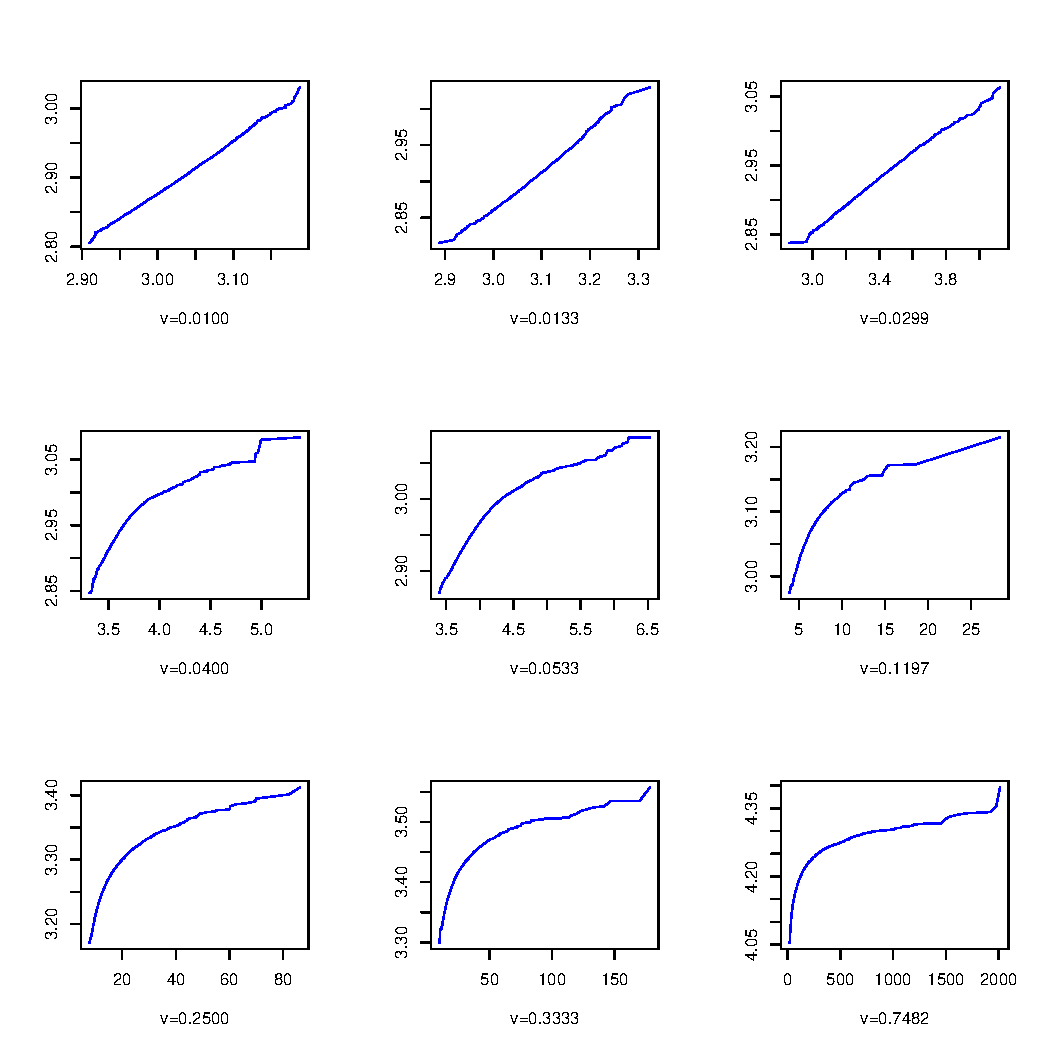
\includegraphics[scale=0.5]{../r/eigmax_TW_q0dot5.pdf}
  \caption{\small \it Comparison of the largest eigenvalue's
    distribution (quantiles along the horizontal axis) with
    Tracy-Widom (quantiles along the vertical axis). $q=N/T=0.5$}
  \label{fig:eig1_TW_q0.5}
\end{figure}

\begin{figure}[htb!]
  \centering
  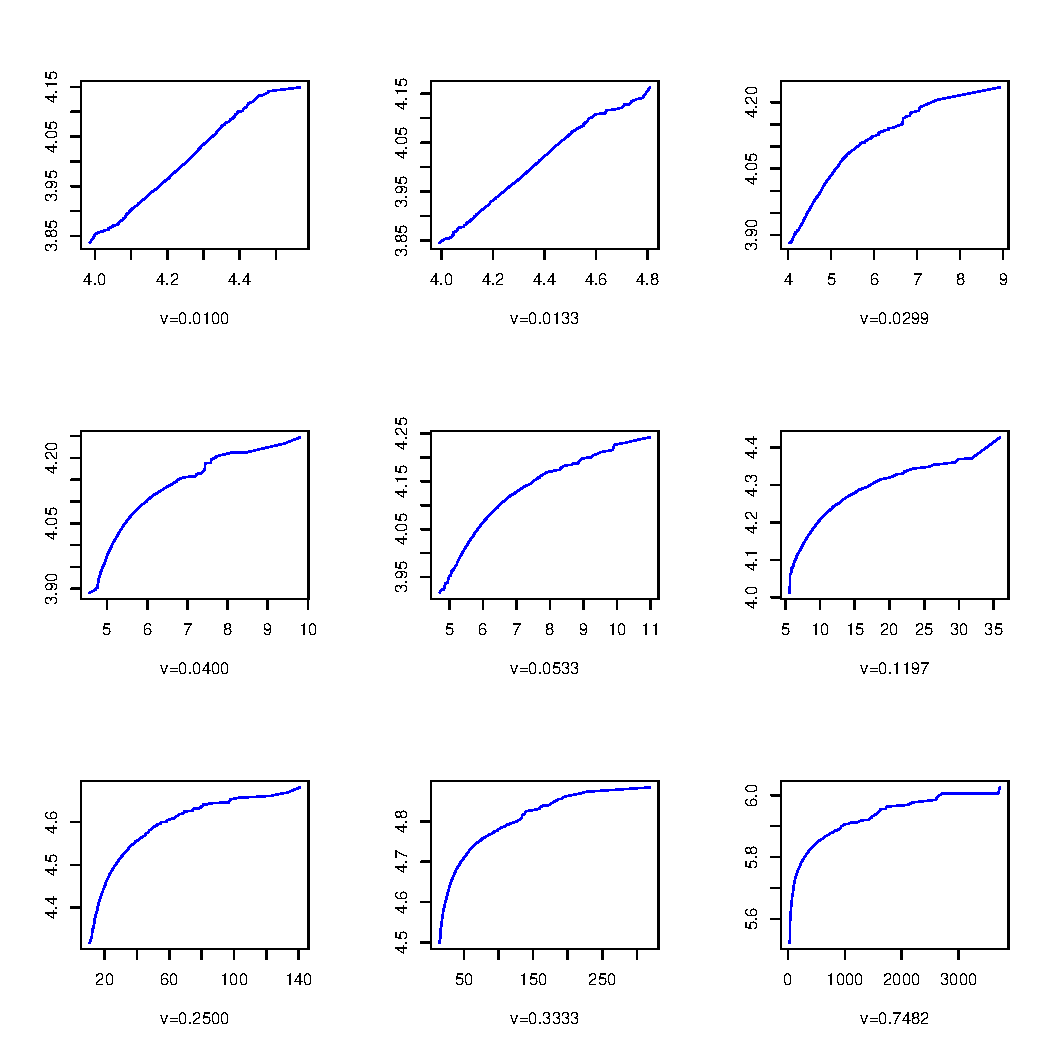
\includegraphics[scale=0.5]{../r/eigmax_TW_q1dot0.pdf}
  \caption{\small \it Comparison of the largest eigenvalue's
    distribution (quantiles along the horizontal axis) with
    Tracy-Widom (quantiles along the vertical axis). $q=N/T=1.0$}
  \label{fig:eig1_TW_q1.0}
\end{figure}

\pagebreak
Figure \ref{fig:eigmax_HillPlot} shows the estimated tail-index of the
maximum eigenvalue distribution against the number of upper-order
statistics used in the estimation (Hill-plot). It is seen that the
region approximately at $(210, 250)$ is stable, suggesting a tail
index of 2.34.
\begin{figure}[htb!]
  \centering
  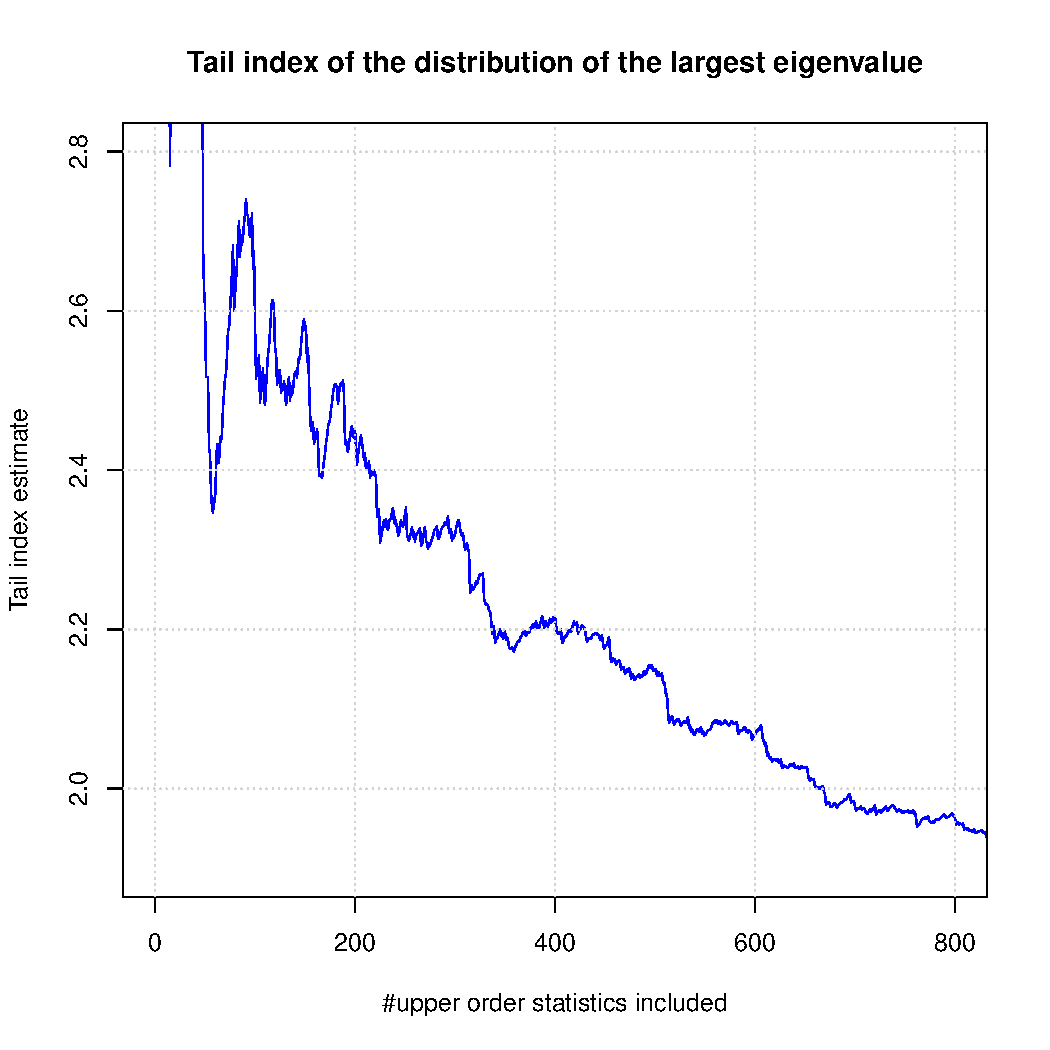
\includegraphics[scale=0.5]{../r/TailIndex_eignmax_q1dot0_v0dot748.pdf}
  \caption{\small \it Hill plot of the largest eigenvalue's
    distribution. $q = 1$, $v = 0.748$.}
  \label{fig:eigmax_HillPlot}
\end{figure}

\pagebreak
Figure \ref{fig:spectral_density} compares the empirical spectral
density with the theoretical density. The value of $v$ used to obtain
the theoretical density is the result of {\it maximum likelihood
  estimation}.
\begin{figure}[htb!]
  \centering
  \subfigure[q = 0.5, v = 0.9415, KL = 0.19]{
    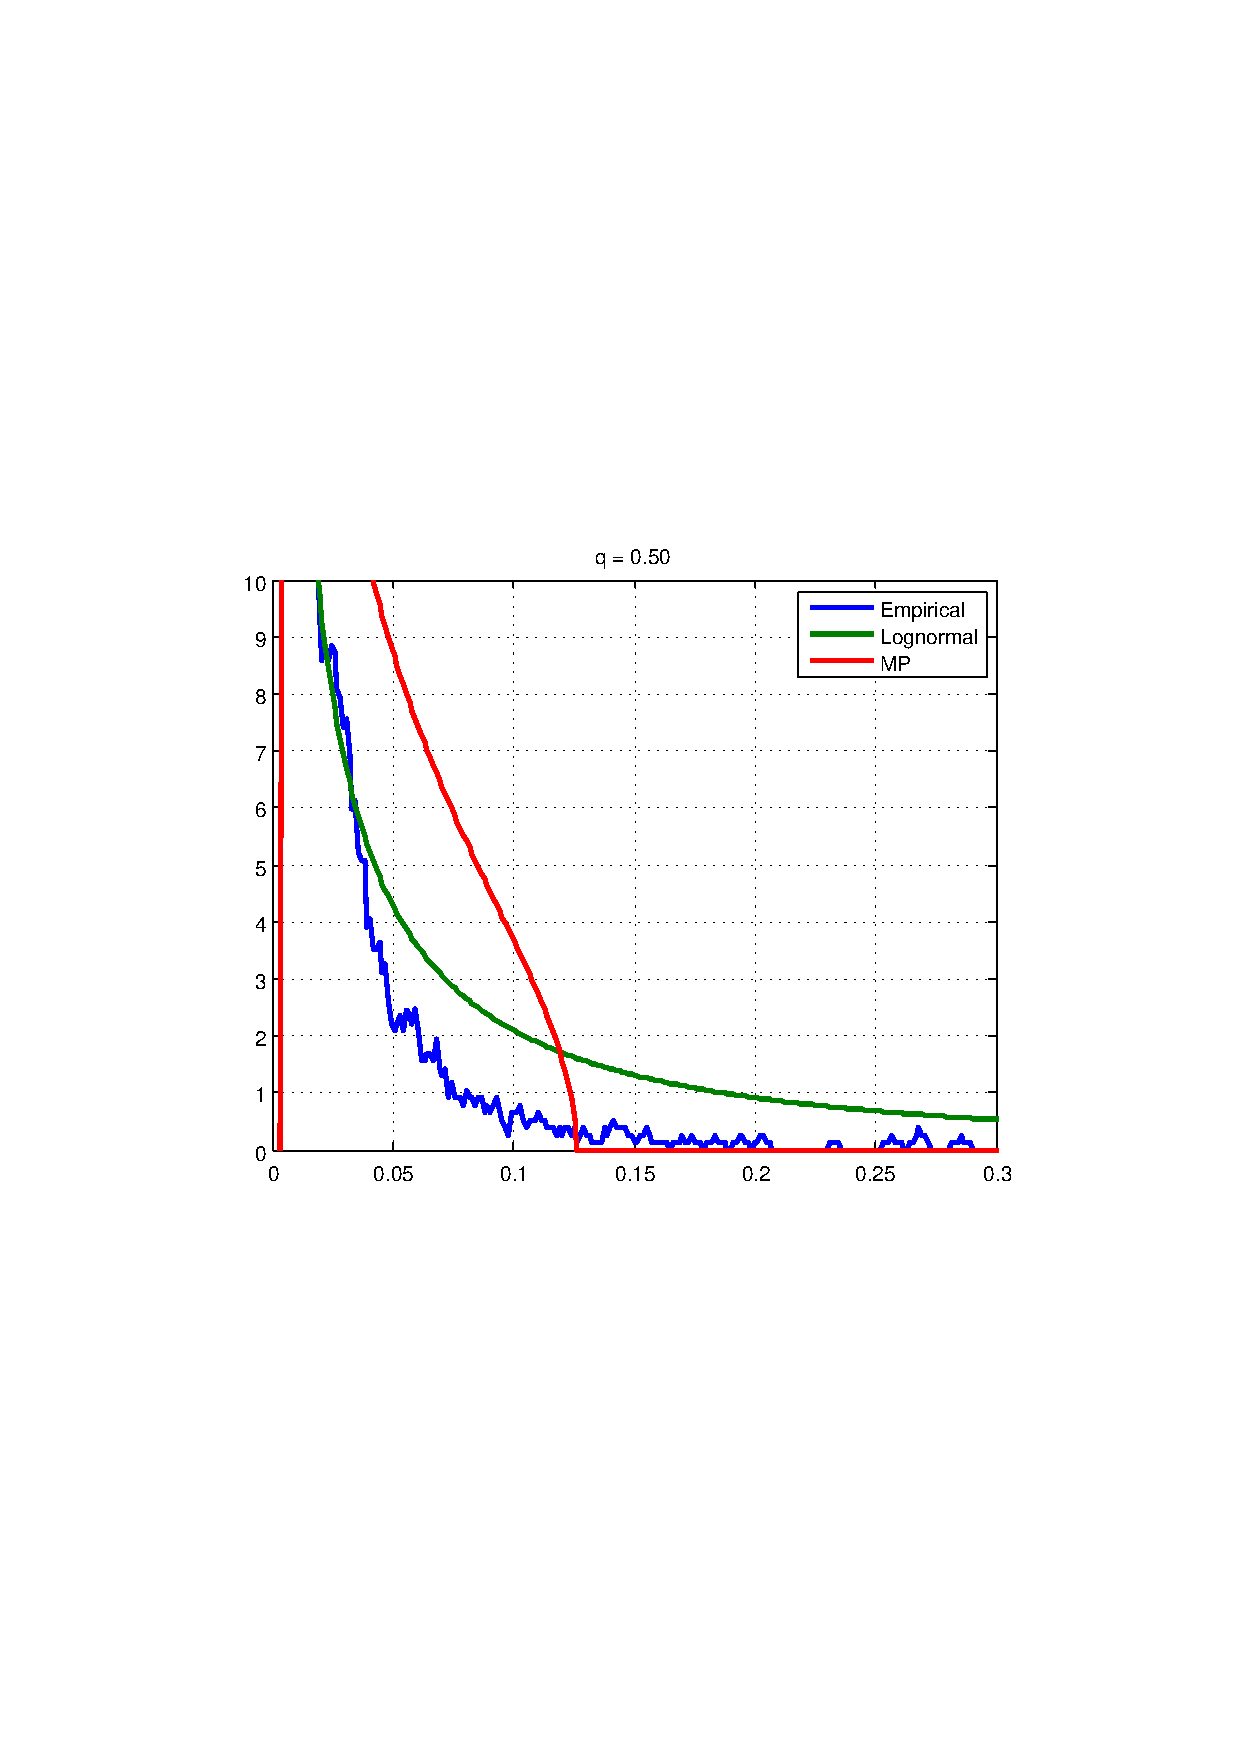
\includegraphics[scale=0.33, clip=true, trim=115 271 109
    204]{../pics/spectral_density_q0dot5.pdf}
  }
  \subfigure[q = 0.65, v=0.8409, KL = 0.15]{
    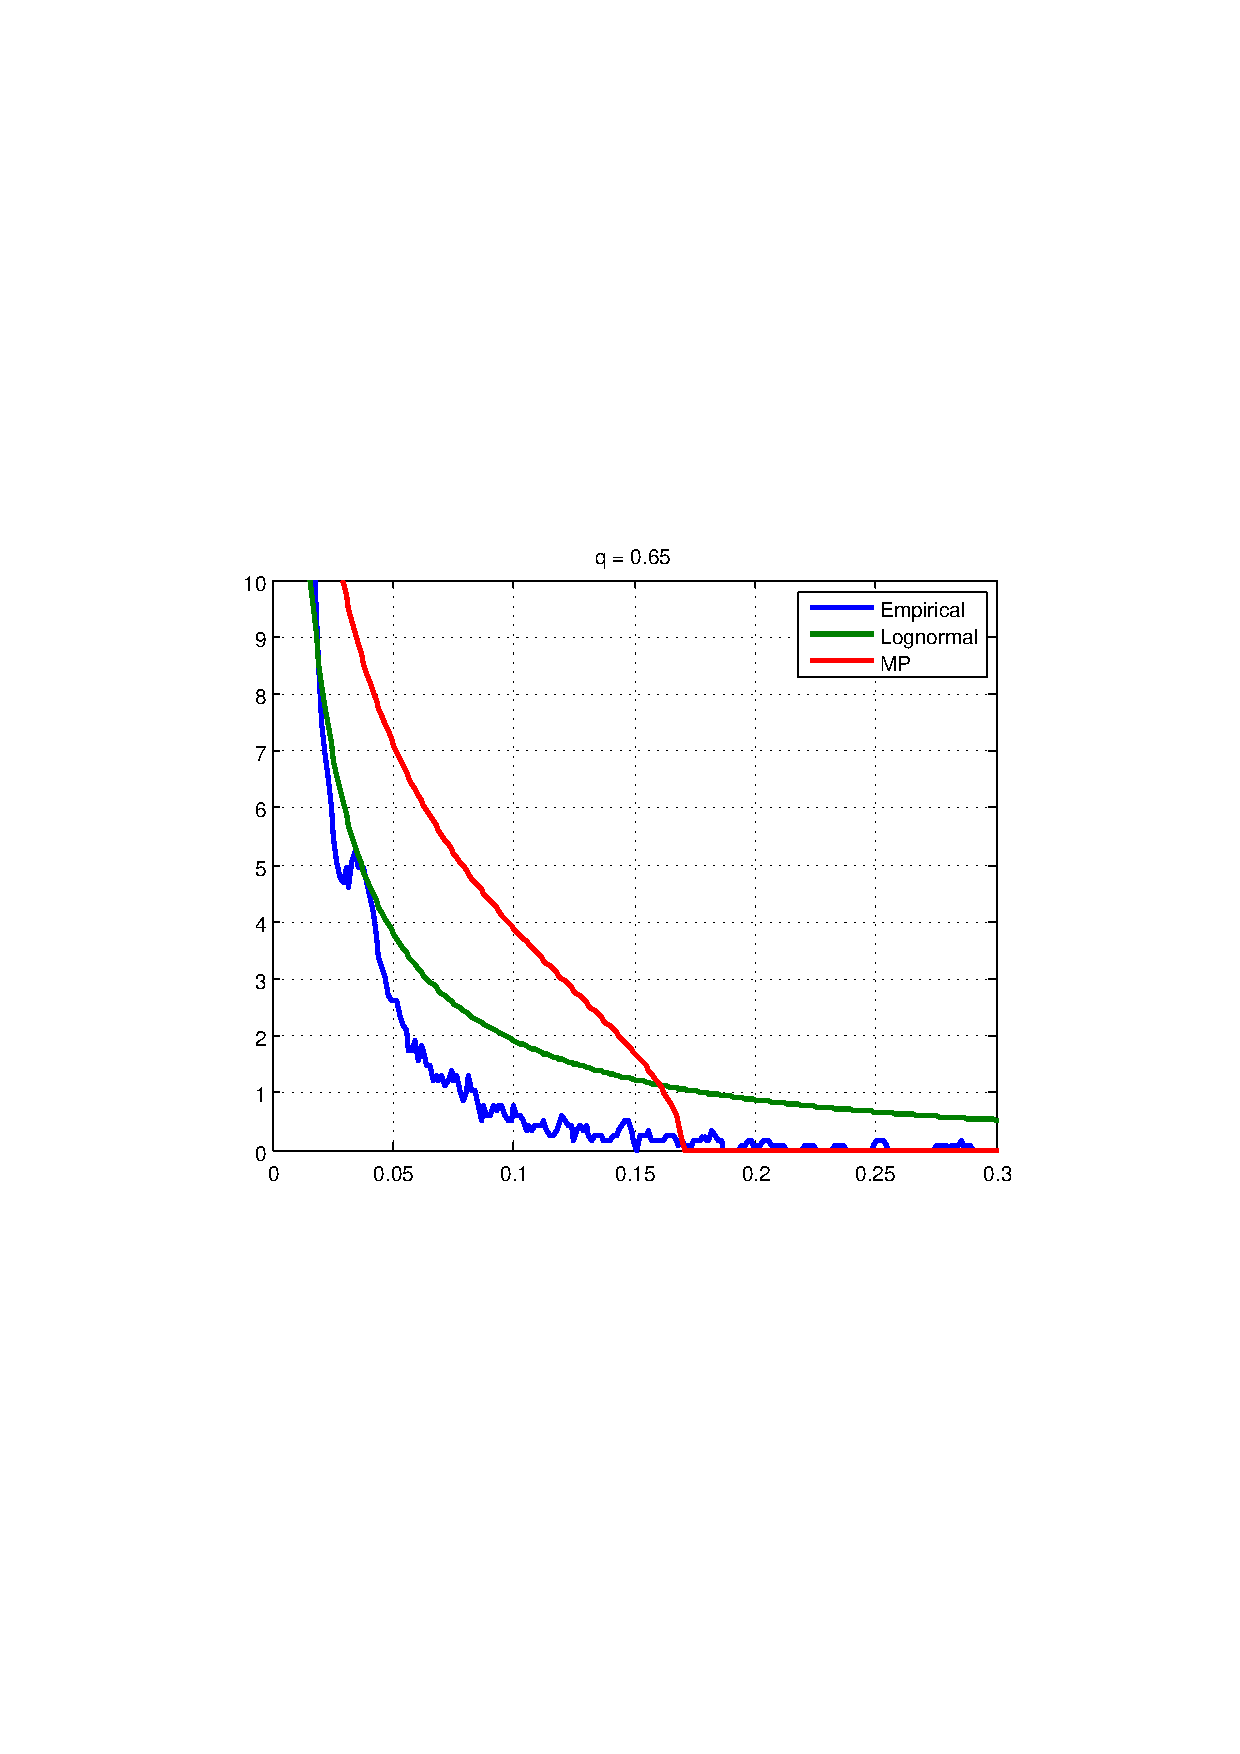
\includegraphics[scale=0.33, clip=true, trim=115 271 109
    204]{../pics/spectral_density_q0dot65.pdf}
  }
  \subfigure[q = 0.8, v=0.8808, KL=0.14]{
    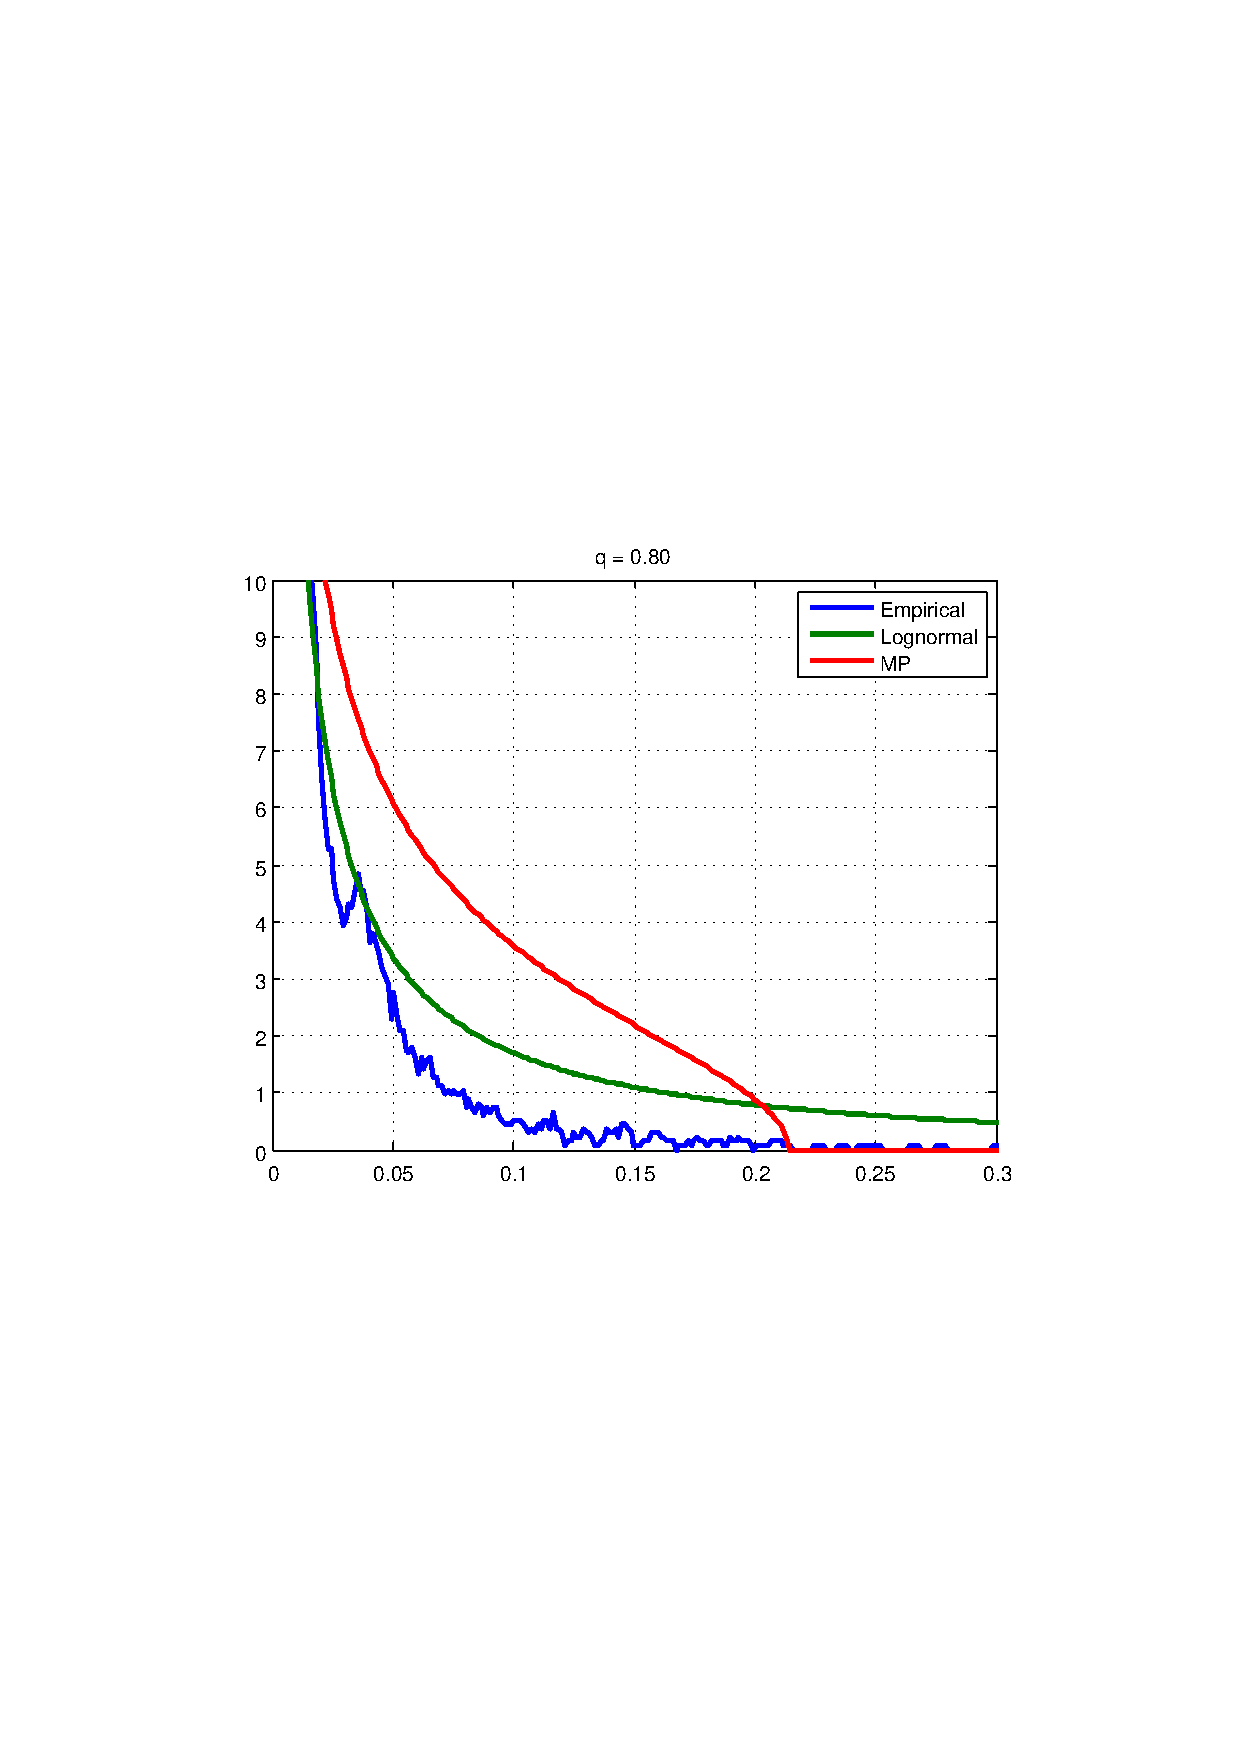
\includegraphics[scale=0.33, clip=true, trim=115 271 109
    204]{../pics/spectral_density_q0dot8.pdf}
  }
  \subfigure[q = 0.95, v=0.8859, KL=0.15]{
    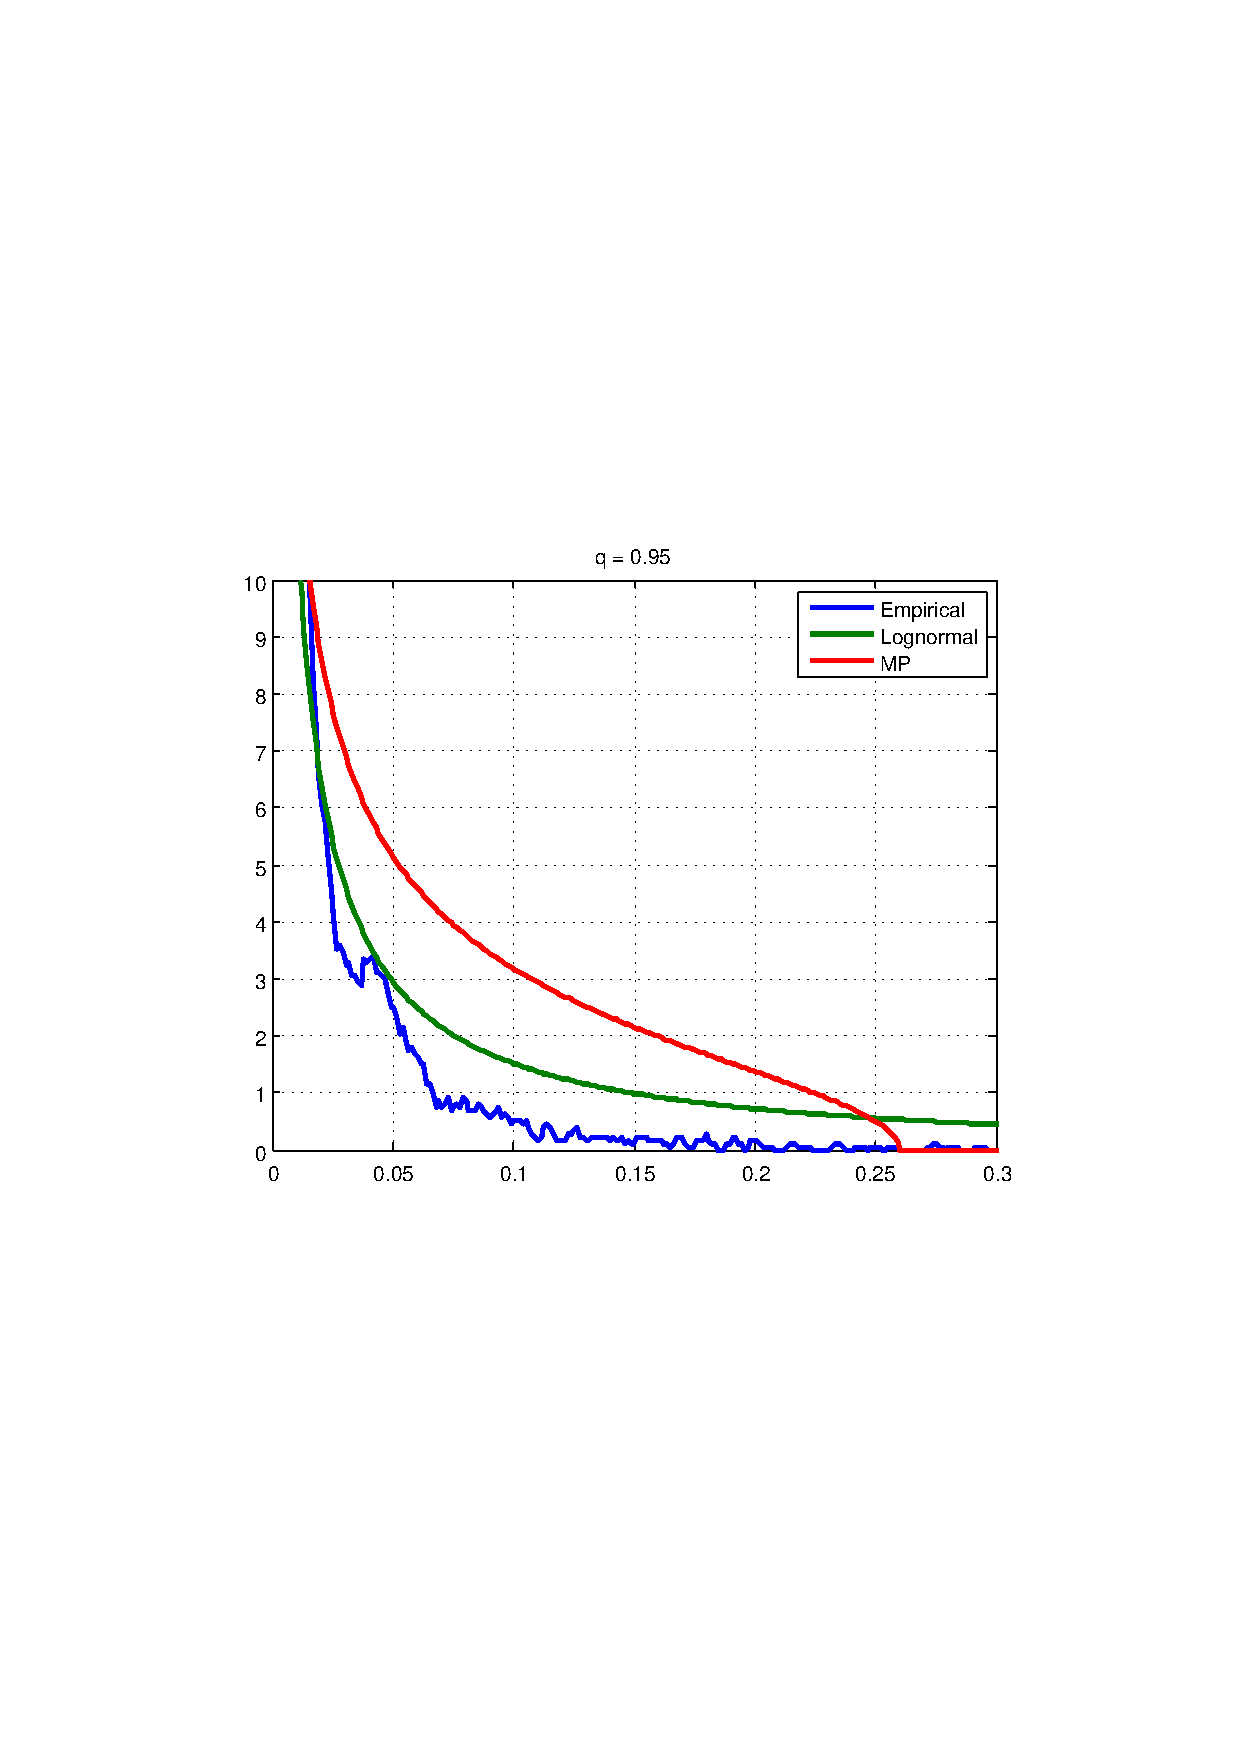
\includegraphics[scale=0.33, clip=true, trim=115 271 109
    204]{../pics/spectral_density_q0dot95.pdf}
  }
  \caption{\small \it Comparison of the empirical and theoretical
    spectral densities. The largest empirical eigenvalue ($\lambda_1$)
    is excluded. The rest is rescaled by $1/\lambda_1$. The
    theoretical density functions are rescaled accordingly. KL
    is the Kullback-Leibler divergence of the theoretical density
    function from the empirical density function. Only intervals on
    which the empirical density is non-zero are included in the
    calculation of KL.}
  \label{fig:spectral_density}
\end{figure}

\pagebreak
Figure \ref{fig:SP500-TailIndices} shows the upper- and lower-tail
indices of 441 stocks in the S\&P-500 index.
\begin{figure}[htb!]
  \centering
  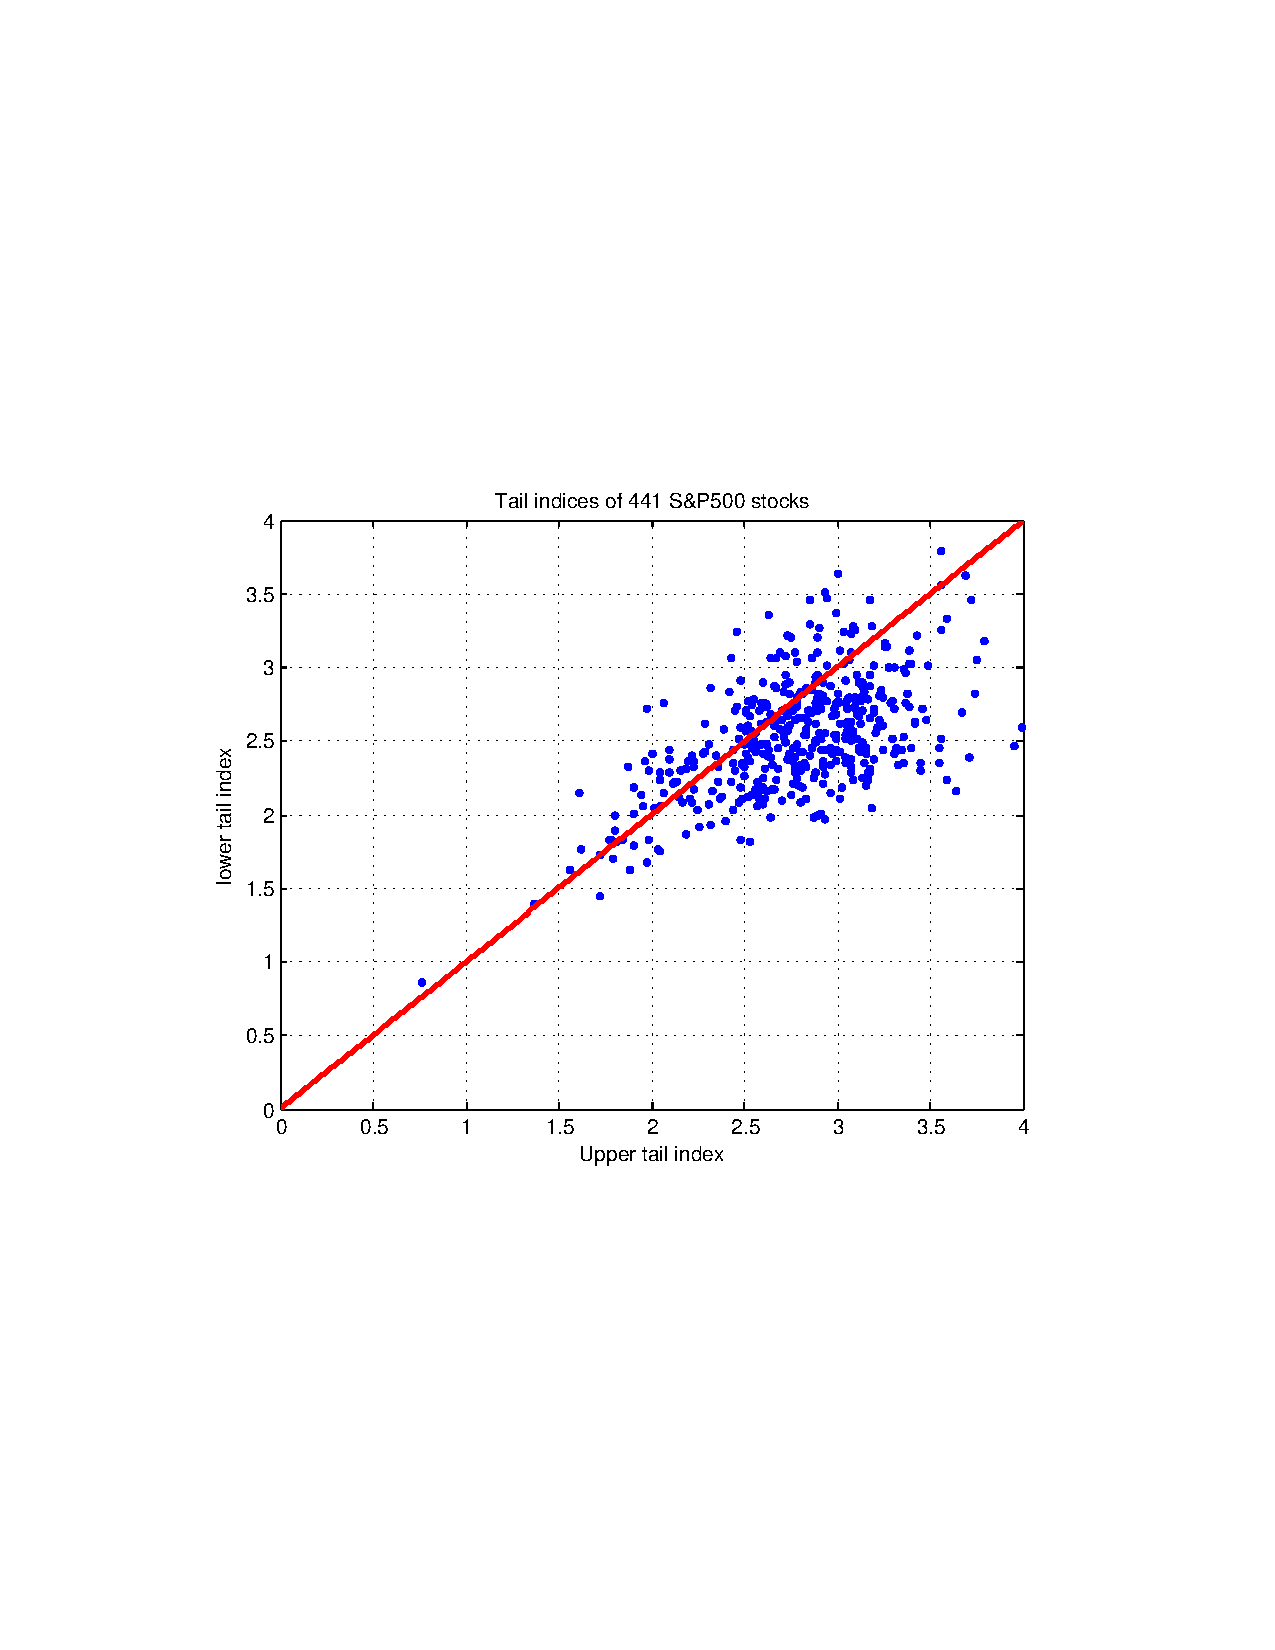
\includegraphics[scale=0.5, clip=true, trim=94 229 115
  121]{../pics/SP500-TailIndices.pdf}
  \caption{\small \it Upper- and lower-tail indices of 441 stocks in
    the S\&P-500 index. The horizontal coordinate of a point in the
    figure is the upper-tail index and the vertical coordinate is the
    lower-tail index.}
  \label{fig:SP500-TailIndices}
\end{figure}


\end{document}
